\documentclass[11pt,a4paper]{article}
\usepackage[margin=2.5cm,includeheadfoot]{geometry}
\usepackage[T1]{fontenc}
\usepackage[utf8]{inputenc}
\usepackage{lmodern}
\usepackage[english]{babel}
\usepackage{microtype}
\usepackage{setspace}
\usepackage{booktabs,tabularx,array}
\usepackage{amsmath}
\usepackage{xcolor}
\usepackage{graphicx}
\usepackage{tikz}
\usetikzlibrary{arrows.meta,positioning}
\usepackage[round,authoryear]{natbib}
\usepackage{hyperref}
\usepackage{fancyhdr}
\usepackage{float}

\hypersetup{colorlinks=true,linkcolor=black,citecolor=blue!45!black,urlcolor=blue!45!black,pdftitle={LLM-as-a-Judge Reliability Lab: Project Summary}}
\setstretch{1.10}
\setlength{\parskip}{0.42em}
\setlength{\parindent}{0pt}
\renewcommand{\arraystretch}{1.14}
\pagestyle{fancy}
\fancyhf{}
\fancyhead[L]{LLM-as-a-Judge Reliability Lab}
\fancyhead[R]{Project Summary}
\fancyfoot[C]{\thepage}
\setlength{\headheight}{15pt}

\begin{document}

\begin{titlepage}
\thispagestyle{empty}
\centering

\includegraphics[width=4.0cm]{../images/Fsr_logo.png}\par
\vspace{0.45cm}
{\Large Faculté des Sciences de Rabat\par}
\vspace{0.12cm}
{\large Master IPS\par}
\vspace{1.55cm}
{\Large\bfseries Projet de Fin d'Etudes\par}
\vspace{1.25cm}
{\LARGE\bfseries LLM-as-a-Judge Reliability Lab\par}
\vspace{0.32cm}
{\large Evaluating Reliability, Biases, and Mitigation Strategies in LLM Judges\par}
\vfill
\begin{minipage}{0.58\textwidth}
\centering
\renewcommand{\arraystretch}{1.65}
\begin{tabular}{@{}r@{\quad}l@{}}
\textbf{Student:} & Ahmed EL BATTAH\\
\textbf{Supervisor:} & Pr. Abdellah IDRISSI\\
\textbf{Academic year:} & 2025--2026\\
\end{tabular}
\end{minipage}
\vfill
{\large Rabat, Morocco\par}
\end{titlepage}

\pagenumbering{arabic}

\section{Introduction and Objective}

Large language models (LLMs) are increasingly used to compare generated answers, rank systems, and support evaluation when full human review would be costly or slow. In a pairwise evaluation, a model receives a prompt and two candidate answers, then selects one answer or returns a tie. This approach is useful, but it raises an important question: how reliable is the model that performs the judging?

An LLM judge may react to the prompt, the answer texts, their order of presentation, the judging protocol, and repeated requests. For this reason, a single agreement score is not enough. A judge can repeat the same decision very consistently while still having only limited agreement with human preferences, or while changing its decision after the two answers are swapped.

In this project, I study LLM judges as measurement instruments. The aim is not to identify one universally best judge. Instead, the project measures several reliability dimensions, examines controlled sensitivities, and evaluates mitigation strategies together with their practical trade-offs. For RQ1, the comparison target is called \emph{human preference reference labels}. These labels are useful references for the study, but they are not treated as ground truth.

\section{Related Work and Research Positioning}

LLM-based evaluation has become an important alternative to large-scale human assessment. G-EVAL showed that a structured LLM evaluation procedure can achieve stronger correspondence with human judgments in its target tasks \citep{liu2023geval}. At the same time, this line of work makes clear that correspondence with humans is only one part of the problem.

MT-Bench and Chatbot Arena helped establish pairwise LLM judging as a practical evaluation setting and examined agreement with human preferences as well as known limitations such as position, verbosity, and self-enhancement effects \citep{zheng2023judging}. Other work has shown that the order of candidate answers can affect an LLM evaluator and has proposed calibration methods for this problem \citep{wang2024fair}. Research on Length-Controlled AlpacaEval similarly shows why answer length must be considered when interpreting automatic preferences \citep{dubois2024length}.

Shi et al. study position bias across several LLM judges and distinguish repetition stability from position consistency \citep{shi2025judging}. Their results show that answer-order sensitivity can differ across judges and tasks, which supports treating repeated fixed-condition decisions (RQ2) separately from answer-order consistency (RQ3).

This literature also suggests that a judge should not be assessed only by the quality of one output. Repetition matters because an evaluation procedure should be stable under the same condition. Presentation matters because a pairwise comparison should not depend on which answer appears first. Mitigation matters because a method that changes agreement may also reduce the number of cases for which it produces a usable decision.

These studies motivate the design of this project, but they do not answer all reliability questions in one place. The present work brings agreement with human preference reference labels, repetition, answer-order swaps, two narrow controlled treatments, source-family association, and mitigation into one controlled and reproducible framework. Each question is measured separately, with its own population and interpretation, rather than being reduced to one overall reliability score.

\section{Research Questions}

The study addresses seven related questions. They are kept separate because they describe different aspects of LLM-judge reliability.

\begin{table}[H]
\centering
\small
\caption{Research questions in plain language.}
\begin{tabularx}{\textwidth}{@{}p{0.08\textwidth}p{0.28\textwidth}X@{}}
\toprule
RQ & Topic & Question \\
\midrule
RQ1 & Human alignment & How often does a judge match a human preference reference label?\\
RQ2 & Repeatability & Does the same fixed evaluation condition produce the same result when repeated?\\
RQ3 & Position sensitivity & Does the mapped decision change when answers are shown in the opposite order?\\
RQ4 & Redundant text & Does one narrow, frozen redundant-text treatment receive a stable advantage?\\
RQ5 & Presentation & Does one controlled list-prefix/presentation treatment receive a stable advantage?\\
RQ6 & Source family & Is there a counterbalanced association between a judge and answers from the same source family?\\
RQ7 & Mitigation & What agreement and coverage trade-offs follow from DUAL\_SWAP and Multi-Judge Consensus?\\
\bottomrule
\end{tabularx}
\end{table}

\section{Dataset and Methodology}

The final study uses a source-corrected canonical dataset built from the MT-Bench human-judgment source snapshot. It contains 80 distinct MT-Bench questions, preserving upstream question IDs 81--160. MT-Bench is multi-turn, so the study represents these questions as 160 turn-level prompt records: 80 first-turn prompts and 80 second-turn prompts. The project therefore contains 80 benchmark questions, not 160 different questions.

The canonical dataset contains 1,568 records. Of these, 1,070 matched the source text exactly and 498 required source correction; none remained unresolved. All 3,355 raw human rows were also reconciled with their upstream reference. This work makes it possible to trace an experimental unit back to the exact prompt and answer texts used in the study.

The final controlled results include four judge families: Claude, DeepSeek, GPT, and Llama. Judges compare answer pairs using three structured outcomes: original answer 1, original answer 2, or tie. Invalid responses, provider failures, and missing observations are recorded explicitly. They are not silently converted into ties or replaced with another model's answer.

Each research question uses a defined experimental unit. For RQ1, the unit is a valid comparison with an available human preference reference label. For RQ2, it is a complete repeated-evaluation cell. For RQ3, it is a matched A/B and B/A pair. The other questions use their own matched variants, counterbalanced units, or retained mitigation populations. This is why the denominators are different across the seven results.

\begin{figure}[H]
\centering
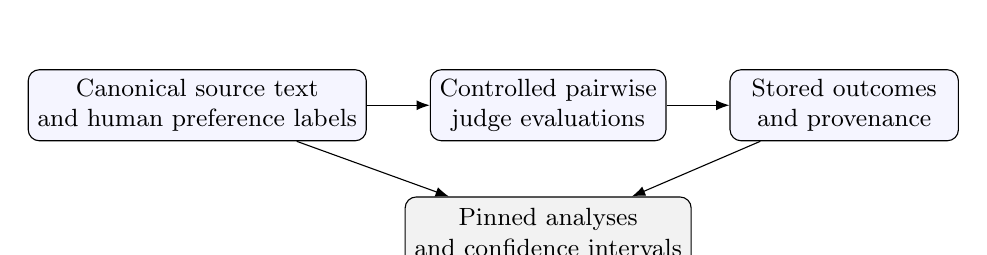
\begin{tikzpicture}[node distance=7mm and 8mm,>=Latex,every node/.style={font=\small},box/.style={draw,rounded corners,align=center,minimum width=29mm,minimum height=9mm,fill=blue!4}]
\node[box] (data) {Canonical source text\\and human preference labels};
\node[box,right=of data] (evaluation) {Controlled pairwise\\judge evaluations};
\node[box,right=of evaluation] (records) {Stored outcomes\\and provenance};
\node[box,below=of evaluation,fill=gray!10] (analysis) {Pinned analyses\\and confidence intervals};
\draw[->] (data)--(evaluation);
\draw[->] (evaluation)--(records);
\draw[->] (records)--(analysis);
\draw[->] (data)--(analysis);
\end{tikzpicture}
\caption{From exact source text to final controlled results.}
\end{figure}

Several design choices support the analysis. RQ2 repeats the same fixed condition. RQ3 evaluates both A/B and B/A presentations, then maps the choices back to the original answer identities before comparison. RQ4 and RQ5 use frozen controlled answer variants. RQ6 uses a counterbalanced source-family design. RQ7 evaluates two mitigation strategies with different retained populations and comparators.

The answer-order mapping is especially important. A raw response of ``Answer A'' has a different meaning after the displayed answers are swapped. The analysis maps every pass back to the identity of the original answer before deciding whether two passes agree or whether a decisive winner changed. This prevents the swap itself from being confused with a preference for an original answer.

When a metric requires complete or decisive observations, the study uses complete-case analysis. Missing results are not imputed, and the eligibility rule is not loosened to enlarge the sample. Confidence intervals are obtained with the frozen procedure using 10,000 bootstrap iterations. The denominator reported for each result therefore states the population to which that result applies. This makes a zero result, a missing observation, and a valid tie distinct outcomes rather than treating them as the same thing.

The pairwise design is useful because both answers are judged in response to the same prompt. However, pairwise results are still conditional on the selected answer pairs and the judging protocol. The study therefore reports the exact analytical population for each RQ instead of presenting a percentage as if it described every possible prompt or model response. This is also why confidence intervals and coverage are reported alongside the point estimates.

\section{Experimental Platform and Reproducibility}

The project includes a React/Vite dashboard, a FastAPI backend, and a PostgreSQL experiment database. Synthesis and Controlled Experiments show the final controlled RQ1--RQ7 evidence. Leaderboard, Bias Diagnostics, and Qualitative Explorer show historical or exploratory telemetry, while Live Evaluation is a separate manual sandbox and is not part of the final study.

The database keeps the prompt, answer, source-model, judge, condition, pass, and analysis information together. Final analyses are tied to persisted evidence, including the source-corrected records. This keeps the correction history visible and prevents an exploratory display from being treated as a final result.

The platform matters because it keeps each reported metric connected to the observations and protocol that produced it. Canonical data, released database snapshots, evidence packages, and tests allow the completed evidence to be checked without new provider calls. Missing, invalid, tied, and terminal observations remain visible, so a reported denominator reflects the data that were actually usable rather than an assumed complete experiment.

\section{Main Experimental Results}

All values below come from the final source-corrected complete-case full-population analysis. Earlier historical results remain available for audit, but they are not used as the final scientific evidence.

\begin{table}[H]
\centering
\footnotesize
\renewcommand{\arraystretch}{1.12}
\caption{Authoritative final results and their interpretation boundaries.}
\begin{tabularx}{\textwidth}{@{}p{0.12\textwidth}p{0.21\textwidth}p{0.28\textwidth}X@{}}
\toprule
RQ & What was measured & Main result & Interpretation \\
\midrule
RQ1 & Agreement with human preference reference labels & 457/772 = \textbf{59.20\%}; 95\% CI 55.70--62.69\%; $\kappa=0.3230$ & Moderate agreement with the reference labels.\\
RQ2 & Strict fixed-condition repeatability & \textbf{96.53\%} (7,119/7,375; 1,475 cells) & High repeatability under the fixed protocol.\\
RQ3 & Decisive mapped answer-order flips & 96/549 = \textbf{17.49\%}; broader disagreement 193/759 = 25.43\% & Position sensitivity exists and differs across judges.\\
RQ4 & Stable redundant-text treatment wins & 0/682 = \textbf{0.00\%} & Applies only to the tested redundant-text treatment.\\
RQ5 & Stable presentation/list-prefix wins & 0/716 = \textbf{0.00\%} & Applies only to the tested presentation treatment.\\
RQ6 & Stable same-family preference & 81/159 = \textbf{50.94\%}; 95\% CI 42.77--58.49\%; 33.13\% coverage & Association only; aggregate patterns are not uniform.\\
RQ7 (P) & DUAL\_SWAP & 67.84\% to 68.51\%, \textbf{+0.67 pp}; CI -0.17 to +1.68; coverage -21.03 pp & Primary: small, uncertain agreement change and lower coverage.\\
RQ7 (S) & Multi-Judge Consensus & 71.82\% vs 66.80\%, \textbf{+5.02 pp}; CI +4.16 to +5.89; 69.83\% coverage & Secondary: positive result against its own equal-weight comparator.\\
\bottomrule
\end{tabularx}
\end{table}

\subsection*{RQ1: Agreement with human preference reference labels}

Across 772 analytical observations, judges agreed with the human preference reference label in 457 cases: 59.20\% (95\% CI 55.70--62.69\%). Cohen's kappa was 0.3230. This is moderate agreement. The judges capture part of the preference pattern, but disagreement remains common. The descriptive rates differ across the four judge families, so these results should not be read as a universal ranking of models.

Agreement is only one reliability measure. It describes whether a valid judge outcome matches the chosen human reference label on this population. It does not tell us whether the same judge will repeat a decision, whether it will react to answer order, or whether its behaviour will transfer to another benchmark.

\subsection*{RQ2 and RQ3: Repeatability and answer order}

The strict repeated-evaluation result was 96.53\% across 1,475 complete cells. Under the same fixed condition, judges usually repeated their decision. However, when the same answers were swapped, 17.49\% of decisive mapped pairs changed their winner. The broader paired-outcome disagreement rate was 25.43\%. High repeatability therefore did not imply high agreement with human preference reference labels or immunity to answer order.

The order result was not uniform across judges. Some families showed far more decisive flips than others in this controlled setting. This is one reason the project reports both aggregate and judge-level views, while avoiding a broad claim that a particular model family is always more reliable.

\subsection*{RQ4, RQ5, and RQ6: Controlled treatments and source-family association}

Neither narrow controlled treatment produced a stable variant win: RQ4 was 0/682 and RQ5 was 0/716. These results concern the exact redundant-text and list-prefix/presentation variants used in the study. They do not settle broader questions about verbosity or formatting.

The value of these results is their precision. The experiment provides evidence about two predefined changes to otherwise matched material. It does not turn a narrow null result into a general claim that answer length or presentation never affects LLM judgments.

The counterbalanced RQ6 experiment found 81 same-family selections among 159 stable decisive units (50.94\%; 95\% CI 42.77--58.49\%), with 33.13\% coverage. The judge-level results varied substantially. The result is best read as a source-family association within this design, not as causal evidence of self-bias.

\subsection*{RQ7: Mitigation strategies}

DUAL\_SWAP is the primary RQ7 strategy. It filters presentation-inconsistent decisions. In this study, agreement with human preference reference labels changed from 67.84\% to 68.51\% on the matched retained population (+0.67 percentage points; 95\% CI -0.17 to +1.68 percentage points). The change is small and uncertain, while coverage fell from 96.87\% to 75.84\% (-21.03 percentage points).

Multi-Judge Consensus is a secondary RQ7 strategy. It aggregates four independent judge votes under a strict rule and is evaluated against an equal-weight individual-judge comparator on its own retained pairs. Agreement was 71.82\% versus 66.80\%, a +5.02 percentage point difference (95\% CI +4.16 to +5.89 percentage points), with 69.83\% coverage. This is a positive secondary result for that comparator and population. It is not a direct comparison with DUAL\_SWAP.

The two strategies therefore address different operational choices. DUAL\_SWAP checks whether a single judge gives a presentation-consistent result. Multi-Judge Consensus aggregates independent judgments under a strict retention rule. Their estimated effects should not be compared as if they came from the same baseline or the same set of retained units.

\subsection*{How to read the result table}

The table reports the primary result for each question, but the values are not all the same kind of quantity. RQ1 is an agreement rate against human preference reference labels. RQ2 is a fixed-condition repetition rate. RQ3 is a paired flip rate after answer identities have been mapped. RQ4 and RQ5 are stable treatment-win rates, while RQ6 is a counterbalanced same-family selection rate. RQ7 reports changes in agreement together with coverage. The numbers are intentionally not combined into one final score.

Coverage deserves separate attention. A mitigation can look better on the cases it retains while returning fewer decisions overall. For this reason, the DUAL\_SWAP result includes both the small agreement change and the 21.03 percentage point coverage reduction. Similarly, the Multi-Judge result reports 69.83\% coverage for its strict consensus rule. A useful deployment decision needs both pieces of information.

\section{Discussion}

The main lesson is simple: LLM-judge reliability has several dimensions. In this study, the judges were highly repeatable under a fixed condition, yet their agreement with human preference reference labels was moderate and their decisions could change when answer order changed. These findings are compatible. A judge may reproduce the same decision consistently while that decision is sensitive to how the alternatives are presented.

The seven research questions make these dimensions visible. RQ1 measures human agreement. RQ2 measures repeated stability. RQ3 measures position sensitivity. RQ4 and RQ5 test two defined treatments. RQ6 examines a counterbalanced source-family association. RQ7 considers agreement and coverage trade-offs in two mitigation designs. Reporting only one score would hide these differences.

The results also vary across judge families. This is why the project does not claim that one judge is universally best. A useful evaluation workflow should report the aggregate result, the relevant per-judge differences, and the conditions under which the result was obtained.

The mitigation results add a practical lesson. A procedure that keeps only certain decisions can change agreement and coverage at the same time. DUAL\_SWAP has a clear coverage cost in this study, while the positive Multi-Judge finding belongs to a different comparator and retained population. These outcomes are useful for deciding how to design an evaluation workflow, but they are not evidence that bias has been eliminated.

The treatment results are also informative even though their numerators are zero. The study tested a specific duplicated-text treatment and a specific list-prefix treatment. Within these frozen designs, neither treatment received a stable advantage. The appropriate conclusion is narrow: the experiment did not observe a stable treatment win in these populations. It would be inappropriate to extend this conclusion to every form of verbosity or presentation.

\section{Limitations}

Fourteen Claude observations remained unavailable and were not guessed or replaced. They were excluded where complete observations were required, so the analysis uses only observations that meet the eligibility rules for each research question.

The conclusions are limited to this MT-Bench population, the 80 questions and their two turns, the four judge families, stored answer texts, and frozen protocols. They should not be generalized automatically to other tasks, languages, model releases, prompts, or deployment settings. RQ4 and RQ5 cover only their narrow treatments. RQ6 is associational. Finally, the two RQ7 strategies use different populations and comparators, so they cannot support a direct claim that one is superior to the other.

\section{Conclusion}

This project provides a controlled study of LLM judges across human agreement, repeatability, answer-order sensitivity, narrow controlled treatments, source-family association, and mitigation strategies. Its scientific contribution is to examine these dimensions separately and to report the populations, confidence intervals, and limits of the conclusions. Its practical contribution is a reproducible platform that connects exact source text, experimental records, analysis runs, evidence packages, and a transparent dashboard.

For practical use, human preference reference labels should be treated as a comparator rather than unquestionable ground truth. Reliability dimensions should be reported separately, especially agreement, repeatability, position sensitivity, and coverage. Repetition and answer-order checks can reveal weaknesses that a single score hides. Provenance should also be preserved, so a result can be traced to the prompt, answers, protocol, and analysis that produced it. Mitigation should be evaluated together with the coverage it retains.

\bibliographystyle{plainnat}
\bibliography{references}

\end{document}
